
\chapter*{Hasil}
\addcontentsline{toc}{chapter}{Hasil}

Setelah melakukan uji coba didapatkan hasil sebagai berikut


Uji Coba dengan data siswa 

\begin{figure}{h}
    \centering
    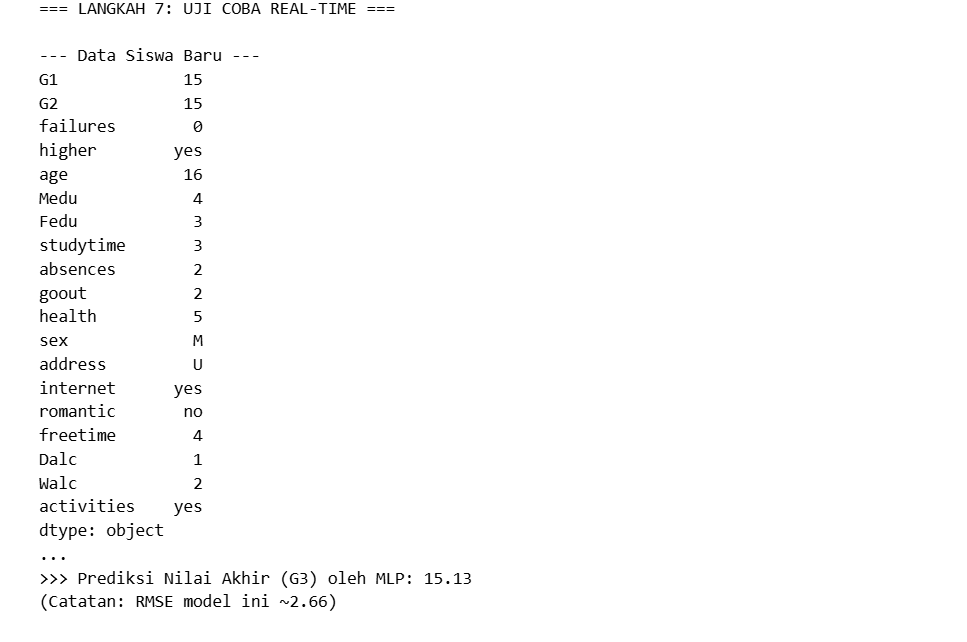
\includegraphics[width=0.8\textwidth]{images/datasiswa2.png}
    \caption{Data Siswa Pertama}
    \label{fig:hasil}
\end{figure}

Disini pada nilai aktualnya nilai G3 siswa adalah 15, dan saat dilakukan uji coba prediksi didapatkan setiap model seperti yang ada pada gambar

\begin{figure}{h}
    \centering
    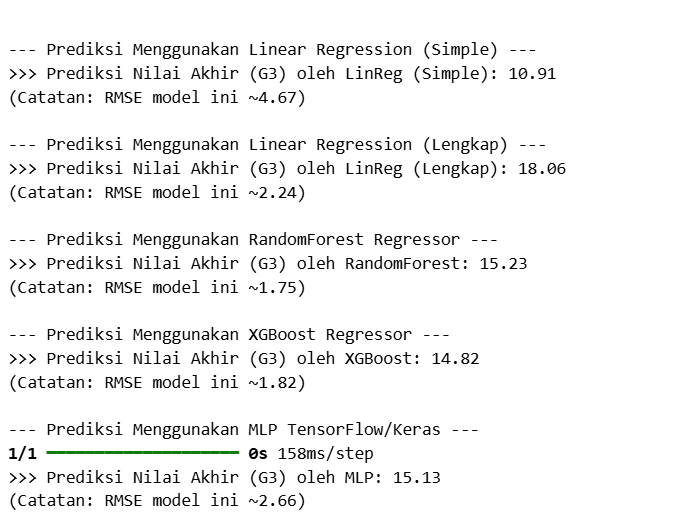
\includegraphics[width=0.8\textwidth]{images/hasil2.png}
    \caption{Hasil Uji Coba Model Pertama}
    \label{fig:hasil}
\end{figure}


Dilanjutkan uji coba dengan data siswa sebagai berikut

\begin{figure}{h}
    \centering
    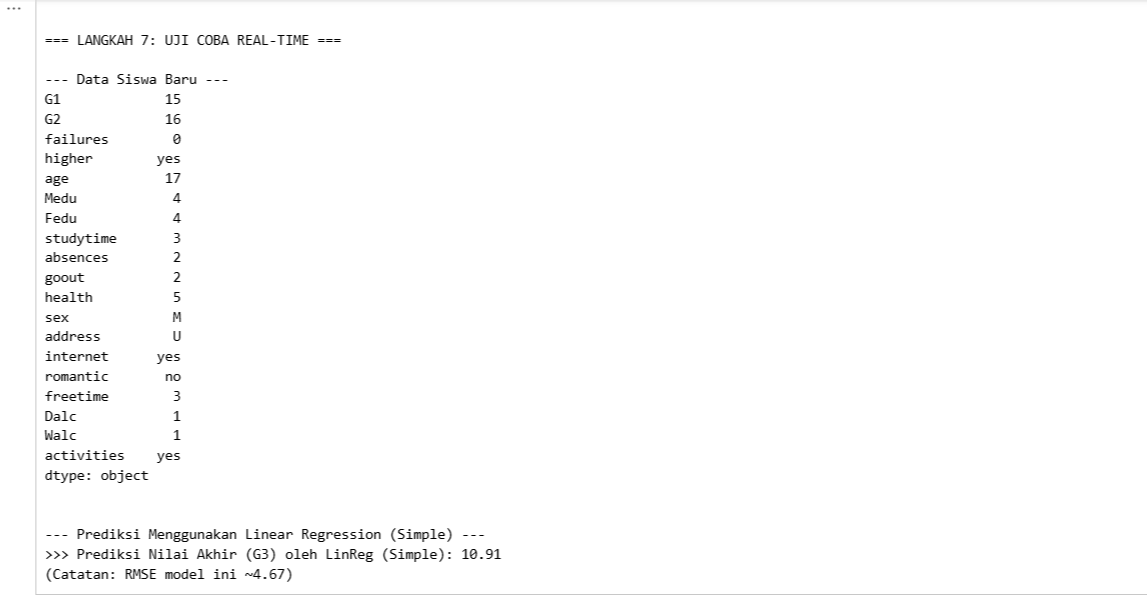
\includegraphics[width=0.8\textwidth]{images/datasiswa1.png}
    \caption{Data Siswa Kedua}
    \label{fig:hasil}
\end{figure}

Dengan data siswa sebagai berikut, kami mengasumsikan bahwa siswa tersebut memiliki nilai G3 sebesar 14,5 yang didapat dengan perkiraan secara intuitif
menggunakan heatmap yang ada dan didapatkan hasil seperti ada di gambar 

\begin{figure}{h}
    \centering
    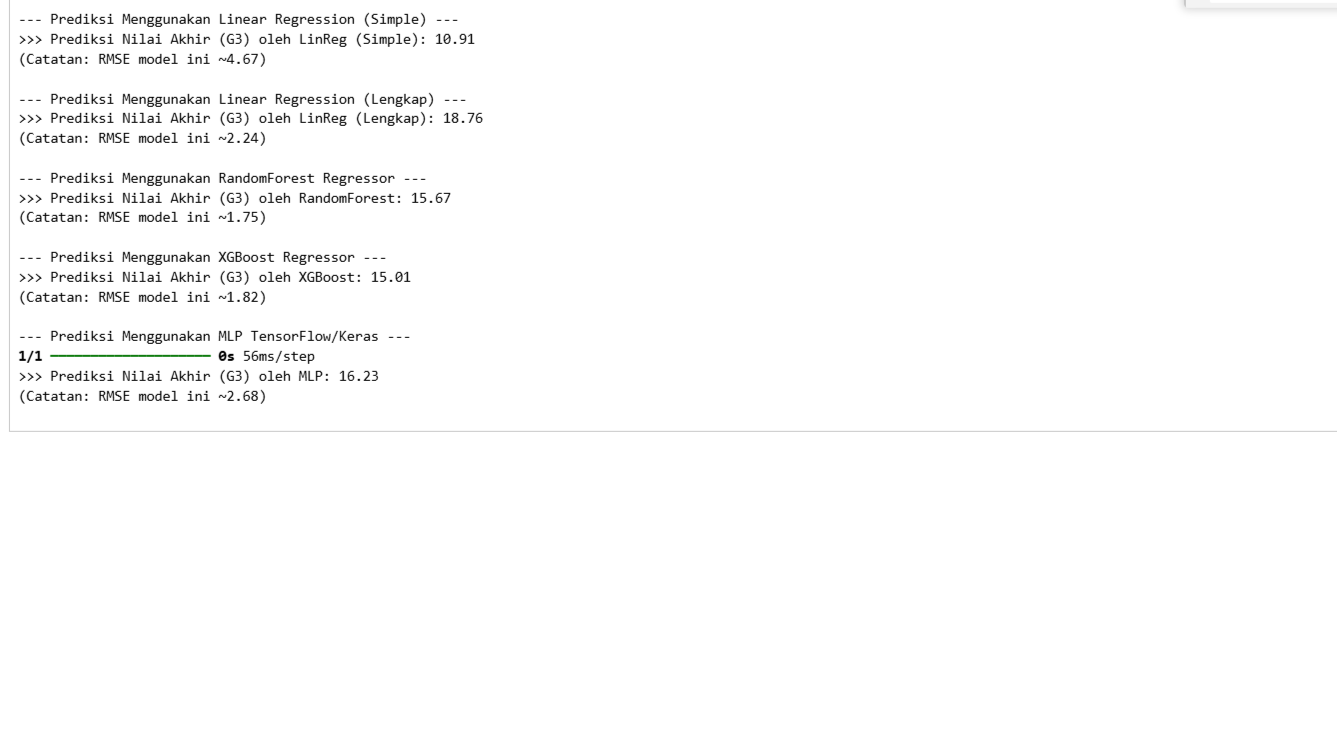
\includegraphics[width=0.8\textwidth]{images/hasil1.png}
    \caption{Hasil Uji Coba Model Kedua}
    \label{fig:hasil}
\end{figure}


Berikut adalah visualisasi untuk RMSE(Root Mean Square Error) dan R-Squared. Dimana nilai RMSE yang baik adalah mendekati 0 dan R-Squared mendekati 1

\begin{figure}{h}
    \centering
    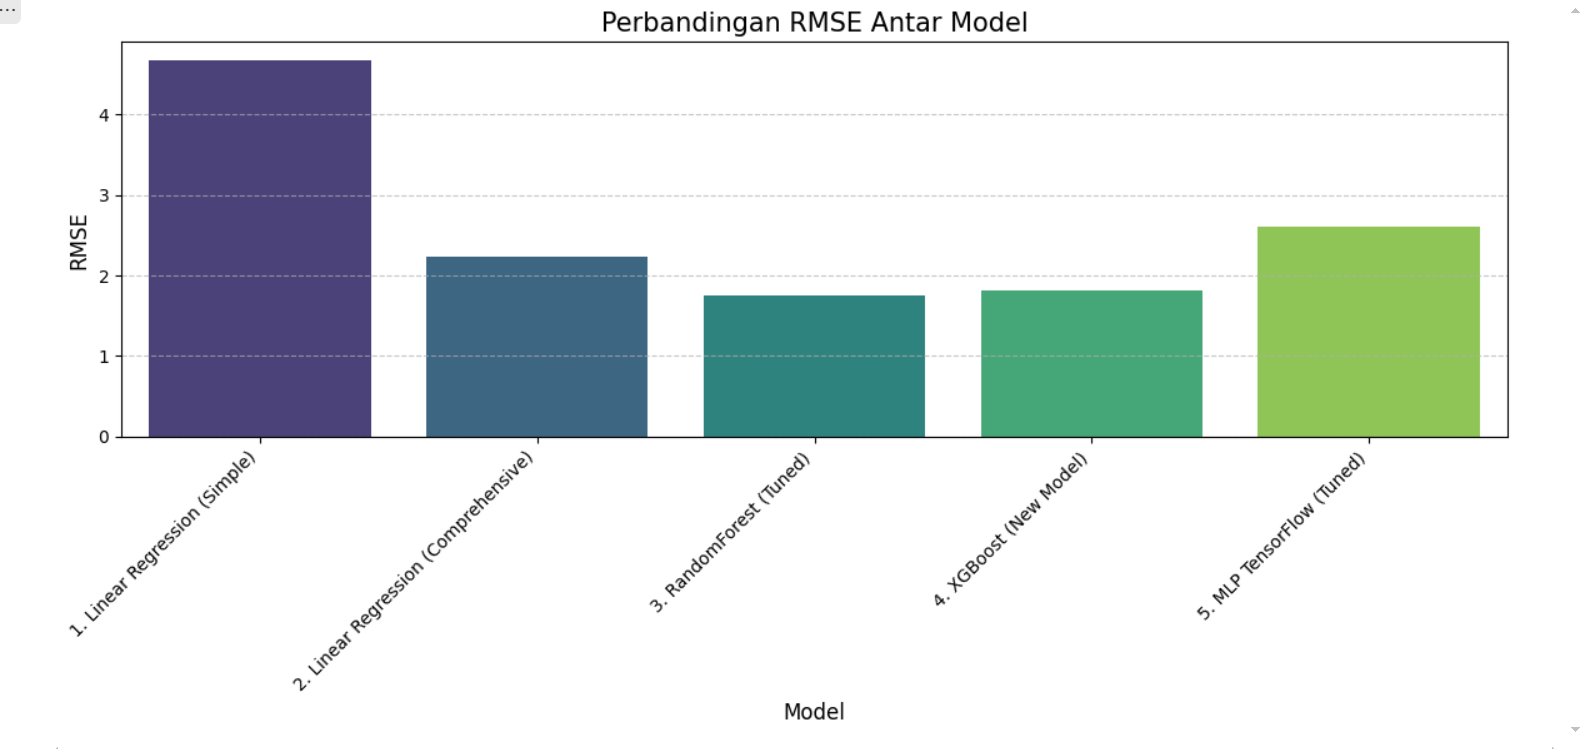
\includegraphics[width=0.8\textwidth]{images/rmse.png}
    \caption{Visualisasi RMSE}
    \label{fig:hasil}
\end{figure}

\begin{figure}{h}
    \centering
    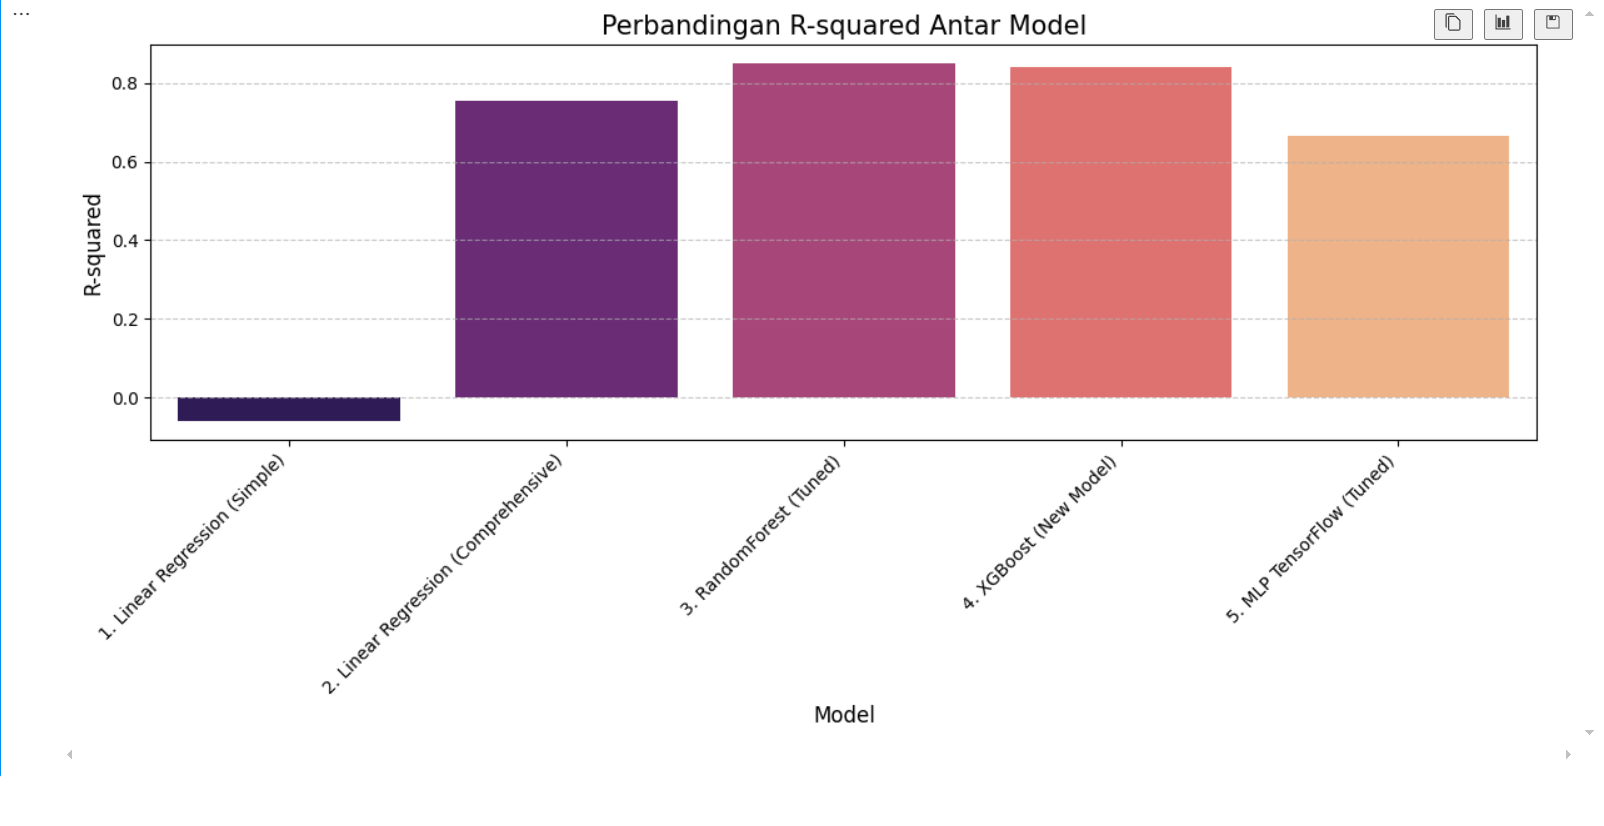
\includegraphics[width=0.8\textwidth]{images/r-squared.png}
    \caption{Visualisasi R-Squared}
    \label{fig:hasil}
\end{figure}

Dari data tersebut RandomForest Regressor mendapatkan nilai RMSE yang lebih rendah daripada semua model yang ada,diikuti oleh XGboost,Linear Regression
dengan fitur yang lengkap, lalu MLP Tensorflow.Nilai RMSE menunjukkan berapa rentang error yang dihasilkan oleh data.Untuk R-Squared RandomForest Regressor
juga yang paling baik diantara model yang ada.R-Squared menunjukkan informasi bahwa bagaimana model tersebut terhadap variabilitas data terhadap model yang 
digunakan. R-Squared menggambarkan seberapa baik model sesuai dengan data yang digunakan.
Secara teknis, RandomForest Regressor mungkin lebih cocok untuk dataset yang relatif lebih kecil dibandingkan MLP TensorFlow dan XGBoost. 
RandomForest umumnya dianggap lebih tidak rumit dalam interpretasi dan implementasi dibandingkan dua model lainnya.\\

Dapat dilihat bahwa performa model RandomForest Regressor adalah model dengan prediksi yang paling akurat dibandingkan dengan model-model lain.
Hal ini dapat terjadi dikarenakan RandomForest Regressor merupakan model yang memang cocok untuk dataset yang lebih kecil daripada MLP tensorflow
dan XGboost. Jika dibandingkan dengan secara teknis RandomForest merupakan model yang paling tidak rumit dibanding ke 2 model tersebut. RandomForest
Regressor bekerja dengan membuat decision tree secara paralel dengan memilih sebuah random data dan dari decision tree yang sudah dibuat secara paralel
nilai prediksi dari setiap decision tree tersebut akan dirata-rata dan akan mendapatkan hasilnya, XGboost juga masih menggunakan decision tree
namun dengan cara memperbaiki kesalahan berulang kali dari decision tree sebelumnya untuk penjelasan simpelnya, untuk MLP Tensorflow sendiri merupakan
salah satu model jaringan saraf tiruan yang memiliki 3 komponen, yaitu; \textit{Input Layer},\textit{Hidden Layer}, \textit{Output Layer} yang memiliki
cara pemodelan yang kompleks dibandingkan dari RandomForest Regressor dan XGboost. 

Kami juga melakukan visualisasi menggunakan scatter plot

\begin{figure}{h}
    \centering
    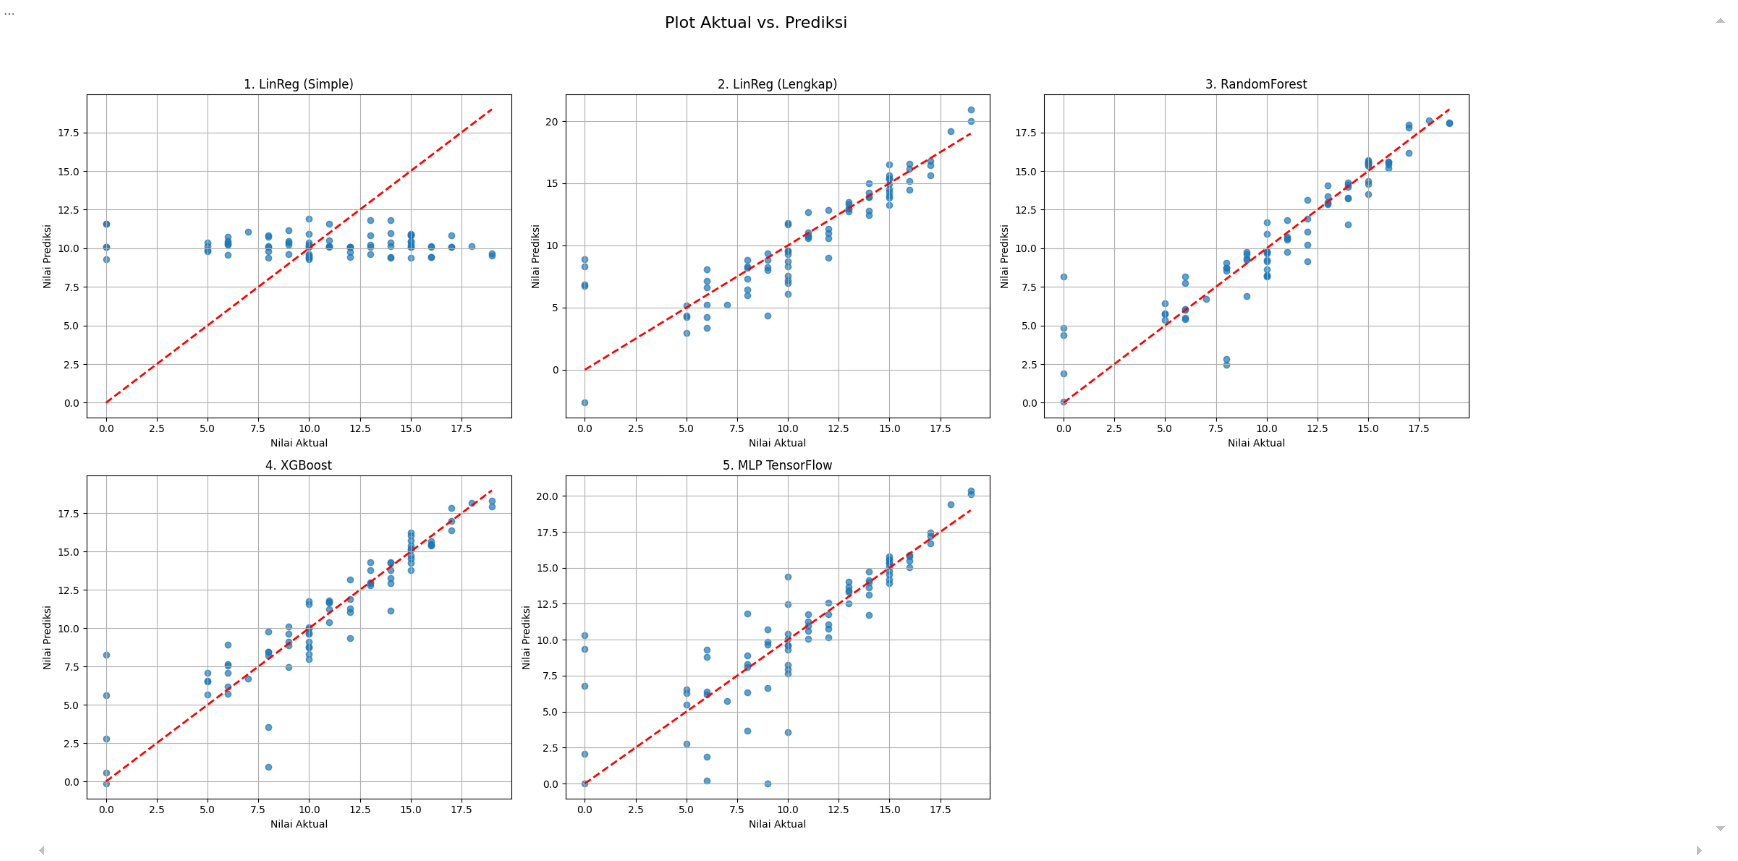
\includegraphics[width=0.8\textwidth]{images/scatter_plot.png}
    \caption{Visualisasi Scatter Plot}
    \label{fig:hasil}
\end{figure}

Dari visualisasi scatter plot yang membandingkan nilai aktual dengan nilai prediksi untuk setiap model, beberapa wawasan penting dapat ditarik 
mengenai performa dan karakteristik setiap algoritma. Idealnya, titik-titik pada scatter plot harus terkonsentrasi rapat di sepanjang garis 
diagonal merah (y=x), menunjukkan bahwa nilai prediksi sangat mendekati nilai aktual.

Model RandomForest Regressor dan XGboost menunjukkan performa yang paling baik dalam visualisasi ini. Titik-titik data 
untuk kedua model ini tampak paling padat dan terpusat di sekitar garis diagonal. Ini mengindikasikan bahwa baik RandomForest maupun XGboost mampu 
menangkap hubungan kompleks dalam data dan menghasilkan prediksi yang konsisten dan akurat di berbagai rentang nilai G3. Kerapatan titik di 
sekitar garis menunjukkan bahwa error prediksi (perbedaan antara aktual dan prediksi) cenderung kecil dan terdistribusi merata.

Sebaliknya, model Linear Regression yang menggunakan fitur baseline menunjukkan sebaran titik yang lebih luas dan menyebar jauh 
dari garis diagonal. Ini terutama terlihat pada nilai-nilai G3 yang lebih ekstrem (sangat rendah atau sangat tinggi), di mana prediksi cenderung 
menyimpang lebih jauh dari nilai aktual. Sebaran yang lebih tersebar tidak merata mencerminkan keterbatasan model linear dalam menangkap hubungan 
non-linear atau interaksi kompleks antar fitur, yang mengakibatkan nilai RMSE yang lebih tinggi dibandingkan model berbasis pohon atau jaringan 
saraf.

Model MLP TensorFlow menunjukkan performa yang kuat, berada di antara Linear Regression dan RandomForest/XGboost. Meskipun titik-titiknya tidak 
sepadat RandomForest atau XGboost, mereka tetap menunjukkan konsentrasi yang baik di sekitar garis diagonal. Ini menegaskan bahwa MLP adalah 
model yang efektif dan mampu memberikan prediksi yang cukup akurat, meskipun dalam kasus ini RandomForest sedikit unggul.

Secara keseluruhan, scatter plot ini secara visual mengkonfirmasi metrik evaluasi yang disajikan sebelumnya. Model-model yang memiliki nilai 
R-squared tinggi dan RMSE rendah (seperti RandomForest dan XGboost) ditunjukkan dengan titik-titik yang sangat dekat dengan garis ideal, sementara 
model dengan metrik yang kurang baik menunjukkan sebaran yang lebih lebar. Visualisasi ini juga membantu mengidentifikasi rentang nilai di mana 
suatu model mungkin berkinerja kurang baik atau di mana terdapat outlier prediksi.


